\subsection{SMP}
Inside each node of a cluster, one can found several processors.
%
These processors often share all resources of the motherboard, this include IO and memory.
%
The way to interconnect all processors with elements of the motherboard can differ.
%
In SMP architecture, all processors are connected to a data bus and a bus arbiter choose with processor can do a memory access (Fig.~\ref{fig:smp}).
%
This design doesn't scale in performance when the number processor grow up.
%
The bandwidth is shared by all processors and the bus arbiter become a bottleneck.
%
Worst, the latency of a memory access depends on the congestion of the bus.

%   (-_-)   %
\begin{figure}[!ht]
        \centering
        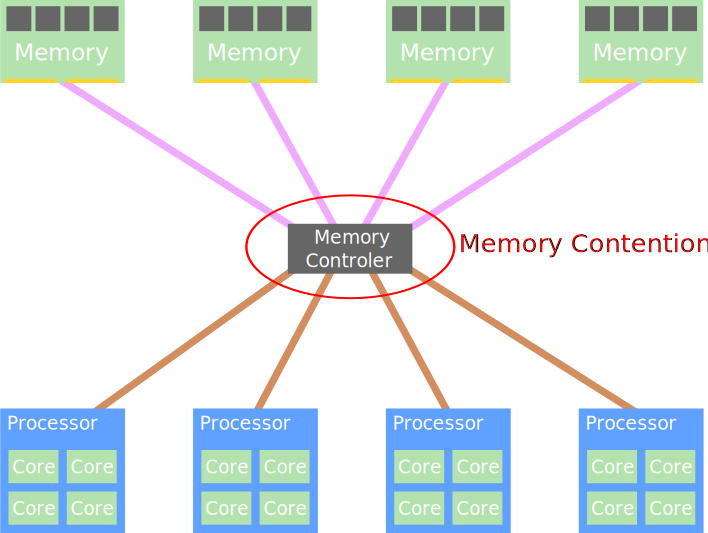
\includegraphics[width=0.8\textwidth]{smp}
        \caption{Overview of an Uniform Memory Access architecture}
        \label{fig:smp}
\end{figure}
